\providecommand{\sumEt}{\ensuremath{\sum E_T}\xspace}
\providecommand{\sumEtring}{\ensuremath{\sum_{\eta-ring} E_T}\xspace}
\providecommand{\sumEtEB}{\ensuremath{\sum_{EB} E_T}\xspace}

\chapter{ECAL energy reconstruction and calibration}

In this chapter the reconstruction and calibration of the energy measured by the ECAL
is presented. Photons are detected only by the ECAL and the analysis sensitivity strongly depends
on the ECAL energy resolution, furthermore some of the variables used to discriminate photons
from jets (see Section~\ref{sec:dipho_selection}) also relies on ECAL information and the stability
over the whole data-taking of such variables is important to ensure an optimal selection efficiency.

\section{Energy reconstruction}
\label{sec:ecal_reco}
A photon or electron entering the ECAL produces a shower in the \PbWO crystals. The energy of
these electromagnetic showers is deposited in crystal matrices. On average the electrons/photons
leave $94\%$ of their total energy in a $3\times3 $ crystal matrix and $97\%$ of their total energy in a $5\times 5$
crystal matrix surrounding the crystal hit by the particle.
Electrons are reconstructed combining ECAL and tracker measurements [59],
while the photon reconstruction relies only on the ECAL [60].

Since the electromagnetic shower generated by a photon or electron span more than one crystal the
energy reconstruction involves both the measurement of the scintillation light in the crystals as well
the clustering of signals originated by the same particle. The clustering takes into account
also bremsstrahlung and photon conversion processes that take place in the tracker and which, due to the
intense magnetic field, spread the energy deposition along $\phi$.
The clustering algorithm [127,128] begin first with the formation of
``basic clusters'', corresponding to local maxima of energy deposits. The basic clusters are then
merged together to form a ``supercluster'' [113], which is extended in $\phi$, to recover the radiated energy.
The different geometric arrangement of the crystals in the barrel and
endcap regions implies that a different clustering algorithm is used for two regions. The algorithms do not
make any hypothesis as to whether the particle originating from the interaction point is a photon
or an electron, consequently electrons from \Zee events can provide excellent measurements
of the photon reconstruction and identification efficiencies, and of the photon energy scale and
resolution. The clustering algorithms achieve a rather complete ($\sim 95\%$) collection of the energy
of photons and electrons, even those that undergo conversion and bremsstrahlung in the material
in front of the ECAL.
The energy in a supercluster can be expressed as:

\begin{equation}
  E_{e,\gamma} = F_{e,\gamma} \cdot \left[ G \cdot \sum_{i} ( S_i(t)\cdot C_i \cdot A_i ) + E_{ES} \right]
\end{equation}
\label{eq:sc_energy}

the sum runs over the crystals composing the supercluster and the terms represent:

\begin{itemize}
\item $A_i$: the signal amplitude in ADC count estimated with the method explained in Section~\ref{sec:signal_reco}.
\item $C_i$: the intercalibration coefficient which equalizes relative differences in the crystals response.
\item $S_i(t)$: the time dependent correction for the loss of transparency explained in Section~\ref{sec:laser}.
\item $G$: the scale coefficient to convert the digital scale measured in ADC count to energy scale expressed in GeV.
  It has two values:
  one for the EB and one for the EE set comparing the scale between data and simulation in \Zee events.
\item $E_{ES}$: Only for electrons or photons in the acceptance region of the ECAL preshower the energy measured
  by the ES is summed to that of the ECAL supercluster.
\item $F_{e,\gamma}$: supercluster energy correction. Several effect like shower non-containment, pile-up and
  loss of energy in the tracker are corrected with a regression technique trained on simulation. The factor also
  takes into account the slightly different shower development of electron and photons.
\end{itemize}

\subsection{Signal reconstruction}
\label{sec:signal_reco}
The scintillation light, emitted by \PbWO , is measured by the photo-detectors as explained in
Section~\ref{sec:cms_calo} and read
out as an analog signal by the front-end electronics. The signal is pre-amplified, shaped
and processed by a multi-gain amplifier. A dynamic range spanning from
approximately 50 MeV to 3 TeV [111] is achieved thanks to three
amplifiers that process the signal in parallel: the amplifiers gains are 1, 6 and 12.
For very high energy photons, the ECAL readout electronic system saturates.
The dynamic range limit is reached when the energy
deposit in a single crystal has a value of about 1.7(2.8) TeV in the barrel (endcaps) and for
non irradiated crystals. The highest, non-saturated signal among the three amplifiers is then digitized by a 12-bit
ADC operating at 40 MHz, ten consecutive samples are read out by the front-end electronics.
% If one of the ten samples is read out from one of the lower gain amplifiers all the following
% samples read with the same gain unless a even lower one is required.


\begin{figure}[!h]
  \centering
  \includegraphics[width = 0.45\textwidth]{figures/ecal/multifit_EB.pdf}
  \includegraphics[width = 0.45\textwidth]{figures/ecal/multifit_EE.pdf}
  \caption{Example of fitted pulses for simulated events with 20 average pileup interactions and 25 ns bunch spacing, for a signal in the barrel. Dots represent the 10 digitized samples, the red distributions (other light colors) represent the fitted in-time (out-of time) pulses with positive amplitude. The dark blue histograms represent the sum of all the fitted contributions \cite{Multifit}.}
  \label{fig:multifit_for_dummies}
\end{figure}

The signal amplitude is reconstructed from the set of ten samples measured for each channel at each event.
The method developed for collisions at 13 TeV and LHC bunch spacing of 25 ns estimates
the in-time signal amplitude and up to nine out-of-time
amplitudes for each signal pulse by a $\chi^2$-minimization via the non-negative-least-squares
technique to the ten digitized samples~\cite{Multifit}, the signal shape used to estimate the contribution of each
energy deposit to each sample is assumed to be the same regardless of when the energy is deposited with respect
the in-time one.
The goal of such approach is to suppress the contributions from OOT energy deposits
to the measurement of the interesting signals.
The out-of-time (OOT) amplitudes corresponds to
energy deposits coming from five bunch crossings that precede the in-time one and four that follow it.
Two examples of a fitted pulse shape for
a simulated event are shown in Figure~\ref{fig:multifit_for_dummies} for the EB and the EE category, respectively.
This method is not used when at least one of the samples is read-out through either the gain 6 or gain 1
amplifiers since a known non-linearity of electronics (slew-rate) introduces a distortion in the signal shape
and therefore bias the estimation of the in-time and out-of-time amplitudes.
In such cases since the in-time signal is usually much larger than the out-of-time ones,
the amplitude of the sixth sample is taken as measurement of the in-time energy deposit.

\section{The laser monitoring system}
\label{sec:laser}
The optical transmission within crystals at the scintillation wavelengths is affected by the production
of color centers under ionizing electromagnetic radiation. This transparency loss process is not permanent,
in fact spontaneous annealing of the colour centers occurs also at room temperature and leads
to a transmission recovery, which is evident when the crystals are not irradiated, such as during
machine-fill gaps or winter stops.
Permanent damage can be induced by hadrons traversing the crystals, its impact on the ECAL energy resolution
is expected to be below the design limits up to 500\fbinv.

Crystals produced for ECAL are optimized to reduce the relative variations in light transmission
during an LHC collision running period to less than $6\%$ for the barrel
crystals (dose rates of 0.15 Gy/h) and less than $20\%$ for the endcaps at $|\eta| = 2.5$ (dose rates of
1.9 Gy/h) [b62].

The laser light pulses are directed to individual crystals via a multi-level optical-fibre distribution
system. The basic operations for barrel geometry are the following: laser pulses transported via
an optical fibre are injected at a fixed position at the crystal’s front face, the injected light is
collected, with the pair of APDs glued to the crystal’s rear face, as for scintillation light from an
electromagnetic shower. Although the optical light path is different from that taken by shower
scintillation photons, this design guarantees that the light transmission is measured in the relevant region.
The underlying principle is similar for ECAL endcaps; however, laser light is injected
at a corner of each endcap crystal’s rear face, and the light is collected (as for scintillation) via
a VPT glued on the crystal’s rear face. The intensity of the injected laser is monitored through a set of PN diodes,
the ratio between the APDs amplitude and the one measured with
the PN diode is used to monitor the transparency variation. Each PN diode monitors a region composed by 100 to 200 crystals.

The energy correction factor extracted by means of the laser monitoring system depends on
the light collection mechanisms of both electromagnetic showers and injected laser.
It is possible to define from first principles a relation between
the APD signal amplitude of a electromagnetic shower ($S$) and the one for injected laser light ($R$) [62].
The demonstration begins considering the average light optical path ($\Lambda$) and the average light attenuation
coefficient ($\lambda$), which is directly related to the light transmission. If we consider a shower, with
initial amplitude $S_0$ , which goes through the crystal, the measured amplitude $S$ is:
\[
  S = S_0 e^{-\frac{\Lambda_S}{\lambda_S}}
\]

a similar relation holds for laser light, although the parameters differ since the optical paths for scintillation
light and laser light are different:
\[
  R = R_0 e^{-\frac{\Lambda_R}{\lambda_R}}
\]

on average the scintillation light production is isotropic and thus
the scintillation light travels a longer path in the crystal before reaching the photo-detector than the
injected laser light, the relation between the two can be written as:
\begin{equation}
  \frac{S}{S_0} = \left(\frac{R}{R_0}\right)^{\alpha}
\end{equation}
\label{eq:light_relation}

where $\alpha = \frac{\Lambda_S \lambda_R}{\Lambda_R \lambda_S}$ is an empiric parameter.

The laser light is injected regularly during the CMS data-taking either during periods between LHC fills or
during the abort gap (a series of several empty bunch crossings during which the special magnets 
are turned on to dump the beam), the response is monitored with a granularity of about 40 minutes.
Three laser wavelength are available: blue (447 nm), green (527nm) and infrared. The blue laser is
preferred since it is the closest one to the scintillation spectrum.

Following Equation~\ref{eq:light_relation}, the correction for the transparency loss is computed as:
\[
  LC(t) = \left(\frac{R(t)}{R(t_0)}\right)^{\alpha}
\]

The reference response $R(t_0)$  is currently set to the one measured at the beginning of 2011 and its history is
reported in Figure~\ref{fig:laser}.
The response $R(t)$ is computed as the ratio between the APDs signal and the PN signal ($APD(t)/PN(t)$), as described above
a PN diode is used to monitor the intensity of the injected light to avoid response variation due to laser instabilities.
Since the absolute intensity of the laser light injected in each crystal is unknown and may vary from channel to channel
(different fibers length, imperfect mechanical and optical matching, ...) it is impossible to estimate the value of $\alpha$
with a single measurement. Furthermore the value of $\alpha$ depends on the absolute transparency of the crystal, which
varies under irradiation.
The average value of $\alpha$ both for barrel and endcaps crystals was determined thanks to a series of measurement perform
at beam test before the CMS installation and in-situ during the first years of data-taking. The limited set of data available
allowed only to determine the average value for the EB and the EE (1.52 and 1.16 respectively).
The majority of the ECAL crystals were produced in
Russia by BCTP while a minor fraction was produced in China by SIC, for these last crystals the value of $\alpha$ was
measured to be 1. From the same studies the spread of the value of $\alpha$ among crystals of the same producer
is known to be around $10\%$. 
An in-situ measurement of $\alpha$ for each single crystal, obtained with data collected during 2016, is reported in Section ???.

\begin{figure}
  \centering
  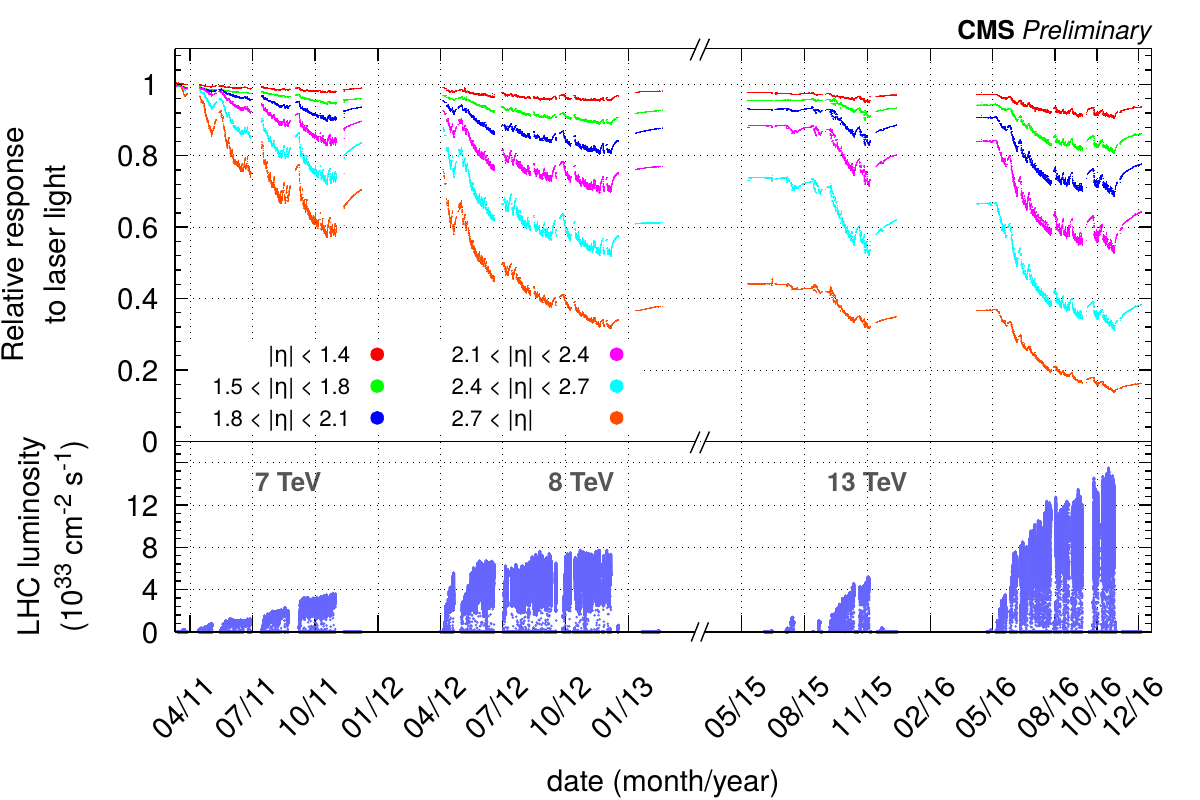
\includegraphics[width = .9\textwidth]{figures/ecal/histories_2011-2012-2015-2016_161212.png}
  \caption{Relative response to laser light (440 nm in 2011 and 447 nm from
    2012 onward) injected in the ECAL crystals, measured by the ECAL
    laser monitoring system, averaged over all crystals in bins of
    pseudorapidity, for the 2011, 2012, 2015 and 2016 data taking periods,
    with magnetic field at 3.8 T. The response change observed in the
    ECAL channels is up to $10\%$ in the barrel and it reaches up to $50\%$ at $\eta\sim 2.5$,
    the limit of the tracker acceptance. The response change is up to $90\%$ in the region closest to the beam pipe
    \cite{laser_and_phisym}.}
  \label{fig:laser}
\end{figure}

\section{ECAL single channel intercalibration and response monitoring}
\label{sec:minchia_la_calibrazione}

The laser monitoring system provide a way to equalize the response over time but does not allow to
correct for absolute response differences among the ECAL channels. The crystal-by-crystal response variation
for crystals at the same $\eta$ ($\eta-ring$) are minimized by means of three techniques, all exploiting collision data:

\begin{itemize}
\item $\Phi$-symmetry: this method is based on the assumption that for a large sample of soft interaction
events (zero-bias) the total deposited transverse energy (\sumEt) is the same for all the crystals in a
$\eta$-ring, any observed asymmetry is attributed to a difference in the response of the crystals.
Intercalibration in $\phi$ is performed by comparing the \sumEt deposited in one crystal
with the total transverse energy collected by crystals at the same value of $\eta$ (\sumEtring).

\item Intercalibration with $\pi_0 and \eta$ mesons:
  In order to take advantage of the high rate of $\pi_0$ decays, a specialized HLT trigger stream has
been developed. In addition, a separate calibration stream has been implemented to select also
$\eta\to\gamma\gamma$ decays. An iterative procedure is used to determine the intercalibration constants.
The $\pi_0$/$\eta$ invariant mass distribution is fitted with a Gaussian function, for the signal, and a
fourth-order polynomial for the background. Then the intercalibration constants are updated
iteratively to correct the fitted mass value in each channel.

\item Intercalibration with isolated electrons: this method selects high energy electrons coming from the decay of
  W and Z bosons. As the previous method it uses an iterative algorithm [63b] that minimizes the difference $E/p - 1$,
  where $E$ is the energy measured by the ECAL while $p$ is the momentum measured with the tracker.
  The crystals belonging to each electron supercluster are inter-calibrated during the iterative procedure.
\end{itemize}

The $\Phi-symmetry$ method is bounded by definition to provide intercalibration coefficients that average to unity
over an $\eta$-ring, for the other two methods instead this requirements is imposed after the intercalibration is completed.
Ring-by-ting response variations are corrected using \Zee events, for each electron/positron the most energetic crystal in the
supercluster determines to which $\eta-ring$ the supercluster belongs to. The ring response is adjusted by fitting the di-electron
invariant mass distribution around the Z peak selecting electrons pairs belonging to different $\eta$-rings.

The three methods have different properties mainly arising from the different energy spectrum used to intercalibrate the ECAL
channel responses.
The $\Phi-symmetry$ method profits from the very large sample of soft collisions and allows to derive a set of intercalibration
constants with just a few hundreds \pbinv but given the low energy of the particles used for the calibration (in the 1-10 GeV range)
it is also affected by a larger uncertainty when compared with the other two methods.
The uncertainty arises from the presence of $\phi$ asymmetric material in front of ECAL
(the tracker system and its services), for these reason the main use of
the $\Phi$-symmetry in the context of intercalibration is to compute correction factor to adjust the intercalibration values
over time for effect such the imprecise knowledge of the $\alpha$ parameter. In this case the effect of the material cancels
out since it does not change with time. A notable exception is when a change in the center of mass energy of the collisions
occurs as explained in Section ??.

The method exploiting $\pi_0$ and $\eta$ is less affected by the presence of material in front of ECAL and
still count on a large data sample but has a poor selection efficiency in the endcaps due to pile-up.

Finally the intercalibration with electrons from W and Z bosons decays although limited by the cross section
of the decay processes is much less affected by systematic effects and over the whole $\eta $ range has the best
precision.

All three methods are also used to monitor the ECAL energy response during the data-taking. The monitored quantities are:
\begin{itemize}
\item $\Phi$-symmetry: the ratio of the intercalibration coefficient at a given time over the reference value ($IC(t)/IC(t_0)$).
%   \begin{equation}
%     F = \frac{\sumEt(t) / \sumEtEB(t)}{\sumEt(t_0) / \sumEtEB(t_0)}
%   \end{equation}
%   \label{eq:eflow_def}
% where \sumEt is the the same sum used for the intercalibration procedure while \sumEtEB is the sum over the chosen period of time
% of all the transverse energy deposited in the EB.
\item $\pi_0$/$\eta$: the peak of the $\pi_0$ invariant mass distribution.
\item Isolated electrons: the $E/p$ ratio.
\end{itemize}

The last two can have a very thin time granularity (several points for each LHC fill) but a spatial granularity of no less
than 200 crystals (the same granularity of the PN diode in the barrel). The monitoring $\Phi$-symmetry

\subsection{The $\Phi$-symmetry method}
\label{sec:phisym}
In this section the $\Phi $-symmetry intercalibration method is presented in details together with the results achieved
during the LHC Run 2 (at 13 TeV center-of-mass energy).

The $\Phi$-symmetry intercalibration method profits from the feature of the CMS trigger that provides the possibility
to record events at a higher rate than that allowed for standard physics data by storing only a fraction of the information
coming from the detector. For the purpose of the ECAL intercalibration only the signals coming from ECAL channels with
and amplitude over a configurable threshold are stored.
The threshold is set to a value that is, on average, equal to 10 times the RMS of the electronic noise.
The noise level depends on the level of radiation damage in the APDs while is constant for VPTs, these leads
to a noise level which raises with time and $\eta$ for channels in the EB (Figure~\ref{fig:ecal_noise}, top)
while is stable in the EE (Figure~\ref{fig:ecal_noise}, bottom).

\begin{figure}
  \centering
  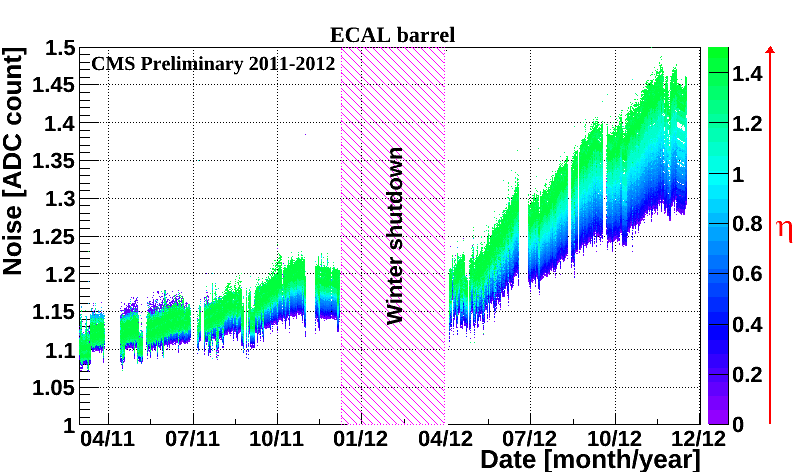
\includegraphics[width = 0.45\textwidth]{figures/ecal/EB_noise_ADC_counts_2011_2012.png}
  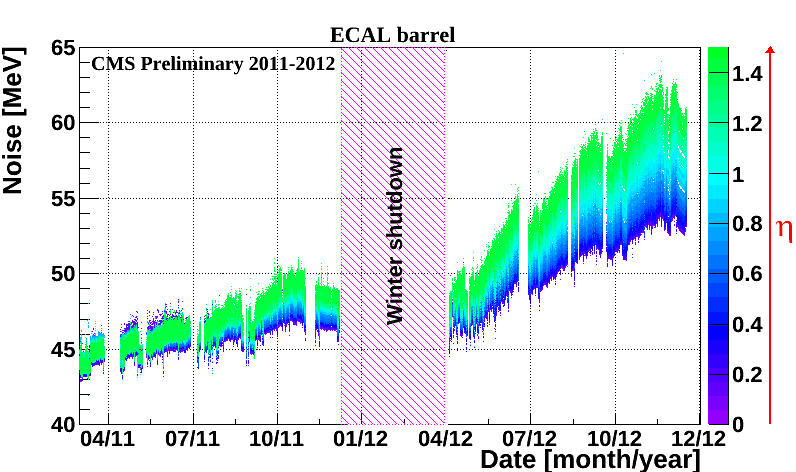
\includegraphics[width = 0.45\textwidth]{figures/ecal/EB_noise_MeV_2011_2012.png} \\
  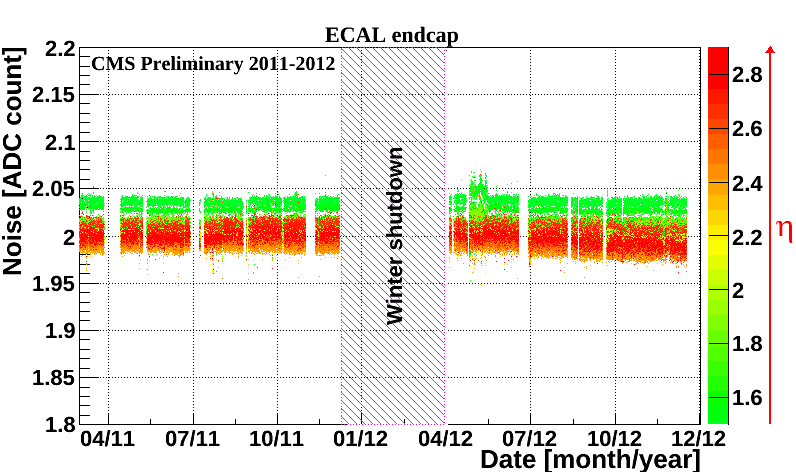
\includegraphics[width = 0.45\textwidth]{figures/ecal/EE_noise_ADC_counts_2011_2012.png}
  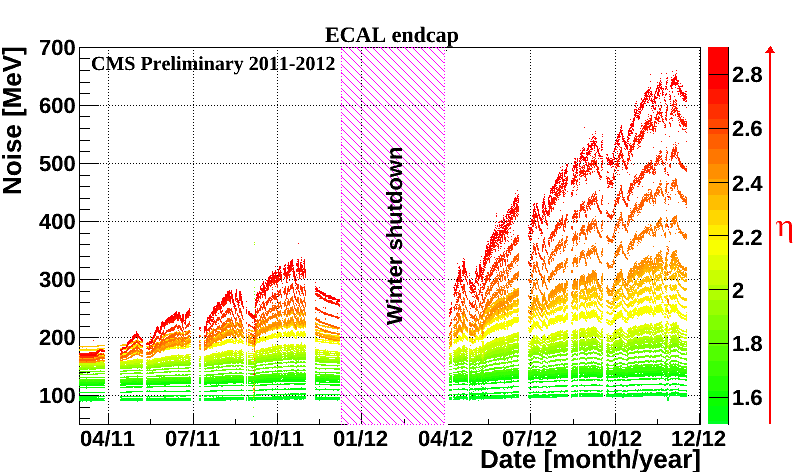
\includegraphics[width = 0.45\textwidth]{figures/ecal/EE_noise_MeV_2011_2012.png}
  \caption{Single channel noise measured on the pre-samples of the laser events taken during
    standard monitoring sequences in 2011 and 2012. The left plot shows the noise in ADC count prior the
    correction for the response loss measured with the laser system while the right one the noise in MeV
    after the correction. Top (bottom) plots includes channels of the ECAL barrel (endcaps)~\cite{ecal_2012}.}
  \label{fig:ecal_noise}
\end{figure}

During 2015 and 2016 the calibration stream recorded events at a variable rate between 1 and 3 kHz with peaks of 20 kHz during
commissioning periods. The rate is kept under control by prescaling zero-bias events (whose rate is almost 40 MHz).

The loss of transparency occurring in the crystals increases the equivalent noise (expressed in GeV) since the
signal amplitude in ADC count is multiplied by the transparency correction derived with the laser system.
For this reason the events used in the intercalibration process
are required to have an energy above a thresholds ($E_{min}$) that takes into
account both the noise level and the loss of transparency and to have a transverse energy not grater then
$E_{min}/cosh(\eta) + 1 GeV$. This higher bound avoids that the energy sum used in the intercalibration is
biased along a certain $\phi$ direction by energetic deposit coming from hard scatterings which might not be
$\phi$-symmetric. The $E_{min}$ depends on the level of irradiation ad was set to $0.8$ GeV in 2015 and $0.9$ GeV in 2016, these
values were optimized to avoid noise induced distortions of the spectrum while keeping the amount of data needed
to derive an intercalibration close to that recorded in a typical LHC fill.
Selecting only deposits in a fixed energy window overestimates any response mis-calibration. This effect in taken into
account by introducing a scaling parameter ($k$) in the intercalibration formula to correct the ratio $\sumEt/\sumEtring$:
\[
  IC = \left( \frac{\sumEt}{\sumEtring}  \cdot \frac{1}{k} \right)^{-1}
\]
$IC$ is the correction factor to be applied to the original intercalibration coefficient in order to obtain the
new intercalibration and is computed for each one of the ECAL channels.
The $k$ parameter is estimated by multiplying the reconstructed energy of each hit by ten known
mis-calibration values ($m_{true} \in [0.9, 1.1]$), the observed mis-calibration is computed as:
\[
  m_{obs} = \frac{\sum E_T(m_{true})}{\sumEt}
\]
and the $k$ parameter is finally extracted as the slope of the linear fit to the distribution of $m_{obs}$ versus $m_{true}$
(Figure ??). The assumption of linearity 
The $k$ parameter depends on the shape of the $E_T$ spectrum so it is computed each time a set of intercalibration
is derived and for each ECAL channel independently, in this way variation of the spectrum induced by the different transparency
conditions are taken into account. Typical values for the $k$ parameter are within 2 and 2.5.

The statistical precision on the intercalibration values is estimated by dividing the dataset by even and odd event number
and by computing the $IC$ for each channel with the two separate sub-dataset.
The $RMS$ of the crystals $(IC_{even}-IC_{odd})/(IC_{even}+IC_{odd})$ distribution divided by $\sqrt{2}$ is quoted as statistical
uncertainty on the $IC$ obtained with the full dataset (the uncertainty value is common for all crystals in the EB and EE).
Typically a new set of $IC$ is derived for each LHC fill (1-2 days) with a relative statistical uncertainty of about $0.4\%$.

\subsection{Energy calibration of the ECAL in 2015}
\label{sec:calib_2015}

After two years of long shutdown LHC resumed operation in 2015 with a higher beam energy 6.5 TeV (instead of 4 TeV) resulting
in 13 TeV of center of mass energy of the p-p collisions. The single channel response of the ECAL, although corrected
for the response variation measured with the laser system, has been corrected with a new set of intercalibration
derived combining the three intercalibration methods.

As explained in Section~\ref{sec:phisym} the $IC$ values derived with the $\Phi$-symmetry method are affected by
a large systematic uncertainty due to the presence of material in front of the ECAL, such effect cancels when taking
the ratio of two sets of $IC$ computed with data collected at different times. This cancellation however does not occur
when the two set of $IC$ are derived with collisions at a different center-of-mass energy.
The effect of the material on the $IC$ is clearly visible in Figure ??: the presence of support structures and services
absorbs part of the particle energy. This translates into a lower than average \sumEt, and consequently higher $IC$ value,
for the ECAL crystals installed behind those structures. The material is however uniform along $\eta$ for crystals within 
the same tracker partitions (barrel and endcaps), so corrections for the impact of material are computed averaging
over $\eta$ the measured $IC$ values at same $\phi$ but for two regions in the EB ($|\eta|<1$ and $1<|\eta|<1.442$).
The $IC$ values are scaled for the average supermodule $IC$ and the correction for the $j-th$ $\phi$-row is defined as:
\[
C_j = \frac{1}{IC_{<\eta >}}
\]
The correction derived in this way are assumed to correct only for crystal-by-crystal variations introduced by the
presence of material in front of ECAL and not for real channel response variations.
The assumption is tested
comparing the correction values derived separately for $\eta <0$ ($C_j^+$) and $\eta > 0$ ($C_j^+$)
(Figure~\ref{fig:material_corrections})
and checking that the pull distribution $(C_j^+ - C_j^-)/\sqrt{\sigma_j^{+ 2}+\sigma_j^{- 2}}$
has a standard deviation equal to $1$ (Figure~\ref{fig:correction_pull}). This confirms that the observed variations
are independent of $\eta$ (in the two region defined above) within uncertainties while a channel mis-calibration
would appear as a systematic variation of the pull.
In total 720 correction values are computed (360 $\phi$-row for two $\eta$ regions) 
The correction computed in this way also correct for gaps in the $\phi$ direction present at the boundary of the ECAL barrel
supermodules (Figure ??). Crystals in supermodules installed in the positive and negative $\eta$ sides of the barrel
have opposite tilt angles, for this reason the effect of the gaps is on the last crystal of a supermodule for the positive
side while on the first one in negative side.
Gaps along $\eta$ are also present as shown in Figure ?? but are irrelevant when computing
the $IC$.

\begin{figure}[h!]
  \centering
  \includegraphics[width = 0.45\textwidth]{figures/ecal/corr_profile_2012_innerEB.pdf}
  \includegraphics[width = 0.45\textwidth]{figures/ecal/corr_profile_2015_innerEB.pdf}\\
  \includegraphics[width = 0.45\textwidth]{figures/ecal/corr_profile_2012_outerEB.pdf}
  \includegraphics[width = 0.45\textwidth]{figures/ecal/corr_profile_2015_outerEB.pdf}
  \caption{Material effect corrections for the barrel inner ($|\eta| < 1$, top row) and outer ($1 < |\eta| < 1.442$, bottom row)
    regions described in the text, the blue (red) curve refers to the negative (positive) $\eta$ side of the barrel.
    Plots on the left(right) side show the corrections for the 2012(2015) $IC$.
    Supermodules gaps affect the $IC$ of the first or last crystal in the supermodule if it is located on the negative or
    positive $\eta$ side respectively. The correction for gaps can be seen in plot as positive correction of about $6\%$
    every 20 $\phi$-rows while. The magnitude of the correction for material effect the larger for 13 TeV collisions (2015)
    than for 8 TeV ones, this can be clearly observed in crystals located behind the main tracker support structures located
    at the 10-th and 190-th $\phi$-rows. The correction for gaps at the supermodule boundaries are on the other end
  independent of the collisions energy since they only depend on the acceptance variation induced by the gaps.}
  \label{fig:material_corrections}
\end{figure}

\begin{figure}[h!]
  \centering
  \includegraphics[width = 0.45\textwidth]{figures/ecal/corr_pull_2012_innerEB.pdf}
  \includegraphics[width = 0.45\textwidth]{figures/ecal/corr_pull_2015_innerEB.pdf}\\
  \includegraphics[width = 0.45\textwidth]{figures/ecal/corr_pull_2012_outerEB.pdf}
  \includegraphics[width = 0.45\textwidth]{figures/ecal/corr_pull_2015_outerEB.pdf}
  \caption{Pull distribution of the correction difference between the positive and negative $\eta$ side of the ECAL barrel.
    Plots in the top and bottom row show the pull for inner ($|\eta| < 1$, top row) and outer ($1 < |\eta| < 1.442$
    respectively. Left (right) side refers to corrections for 2012 (2015) $IC$ set. Crystals located at supermodule
    boundaries are excluded from the pull since the gaps are, in principle, unrelated between the positive and negative
  barrel side.}
  \label{fig:correction_pull}
\end{figure}


The same material induced effects are observed in the endcaps but no way to factorize it from real channel-to-channel
variations has been found and a larger uncertainty has thus been attributed to the $IC$ values derived with $\Phi$-symmetry.

The corrected barrel $IC$ values are shown in Figure ??, the channel-by-channel ratio of the two $IC$ set (computed with
data from the last period of data-taking in 2012 and the first one in 2015) has been used to correct the intercalibration
derived by combining the three methods in 2012 in order to provide a new intercalibration for 2015. The $\eta$-ring
response variations has also been adjusted with the method described in Section~\ref{sec:minchia_la_calibrazione}.

To obtain the final channels intercalibration for EB channels the $IC$ values from the three methods are combined, the final values
for each channel is the weighed average of the three. The weight used for the combination is the uncertainty on the $IC$
measure by each method and is estimated for each $\eta$-ring by computing the variance of the $IC$ difference for each
pair of methods. These variances are assumed to be to sum in quadrature of each method uncertainty consequently,
the precision of each intercalibration set is extracted by solving three simultaneous equations for the three the uncertainties.
The results on the uncertainties are reported if Figure~\ref{fig_ecal_ic_precision}. Taking advantage of the
small statistical uncertainty and the reduced impact of the material the $IC$ derived with $\Phi$-symmetry has the best precision
in all $\eta$-rings. The intercalibration with electrons precision is dominated by the statistical uncertainty which
is smaller at smaller $\eta$.

\begin{figure}[h!]
  \centering
  \includegraphics[width = 0.7\textwidth]{figures/ecal/ICs_precision.pdf}
  \caption{Residual mis-calibration of the ECAL Barrel (EB) channel inter-calibration, as a function of pseudo-rapidity with the dataset recorded during 2015. The red points refer to the inter-calibrations derived with Run1 data, extrapolated to 2015 using the laser monitoring system, and corrected using the $\phi$-symmetry of the low energy deposits in the 2015 dataset. The green points refer to intercalibration constants obtained using photons from $\pi_0\to\gamma\gamma$ decays, while the blue points to that obtained using electrons from W and Z decay .The black points represent the residual mis-calibration of the combination of the three methods (weighted average). The precision of the $\Phi$-symmetry and $\pi_0$ calibrations is at the level of the systematic errors. The precision of the electron calibration is dominated by the statistical errors with the dataset recorded in 2015 (2.6 \fbinv). References: CMS DP 2013/007}
  \label{fig:ecal_ic_precision}
\end{figure}

In the endcaps only intercalibration values from $\Phi$-symmetry and electrons were available and they were combined
without weights.

The energy resolution achieved with final intercalibration, including the ring to ring
correction derived with the method described above, is shown in Figure~\ref{fig:ecal_res_vs_eta}.
The resolution $\sigma_E/E$ is extracted from an unbinned likelihood fit to \Zee events,
using a Breit-Wigner function convolved with a Gaussian as description of the Z boson invariant mass peak.
The resolution is affected by the amount of material in front of the ECAL and is degraded in the vicinity of
the cracks along the $\eta$ direction between ECAL modules (indicated by the vertical lines in the plot)
The resolution, especially in the barrel, improves significantly after a dedicated calibration by using
the transported calibrations derived in 2012 and combining them with the calibrations obtained
from the 2015 CMS dataset (blue points),
compared to the prompt reconstruction using only the unmodified 2012 calibrations (black points). 
The resolution in the central barrel reaches the level achieved in Run1,
while int the endcaps the resolution is still significantly affected by the statistical precision of the calibration
(derived with a dataset equivalent to $2.6\fb$).

\begin{figure}[h!]
  \centering
  \includegraphics[width = 0.7\textwidth]{figures/ecal/EcalEnergyResolutionGolden.pdf}
  \includegraphics[width = 0.7\textwidth]{figures/ecal/EcalEnergyResolutionShowering.pdf}
  \caption{Relative electron (ECAL) energy resolution unfolded in bins of pseudo-rapidity $\eta$
    for the barrel and the endcaps \cite{ecal_dpg_2015}. Electrons from \Zee decays are used.
    The vertical dashed lines indicate module boundaries while the grey band around $\eta = 1.5$ denotes the transition
    between barrel and endcaps.
    The resolution is shown for low (left plot) and high (right plot) bremsstrahlung electrons,
    the categorization is based on the $R_9$ variable ($R9=E_{3x3}/E_{SC}$, where $E_{3x3}$ is the energy
    deposited in the most energetic crystal in the cluster and the 8 surrounding ones while $E_{SC}$ is the total
    supercluster energy as expressed in Equation~\ref{eq:sc_energy})}
  \label{fig:ecal_res_vs_eta}
\end{figure}

The residual differences between data and simulation
are due to the statistical uncertainties (endcaps) and other systematic effects described in \cite{run1_egamma}.
Part of these effects are variation of the response over time that are not corrected using the laser monitoring
system data. During 2016 thanks to a larger dataset these effects have been investigated in more details as
described in the next section.

\subsection{ECAL energy response monitoring in 2016}
Given the relative short break between the two data-taking periods (compared to the LS1)
the calibration obtained with data in 2015, corrected for the response variation
due to transparency gain observed with the laser system, was used as baseline
for the energy reconstruction during the 2016 data-taking period.
The energy reconstruction algorithm described in Section~\ref{sec:ecal_reco} was found to depend on both
the crystal-by-crystal noise level and signal shape used in the fitting procedure, thus a monitoring and prompt adjustment
of both quantities was developed during the data-taking. The energy calibration process described in this section
is based on data reconstructed with the updated and time-dependent reconstruction. 

A drift over time of the energy scale was however observed during the year as variation of the Z boson
invariant mass peak in the di-electron spectrum, together with a constant worsening of the resolution.
As explained in Section~\ref{sec:laser}, the transparency variation observed with the laser system differs
from the one affecting the scintillation light collection by an exponential factor $\alpha$.

The per-crystal $\alpha$ parameter can be measured using the same low energy particles from soft collisions
use for the $\Phi$-symmetry intercalibration method. The measurement is performed by minimizing the $\chi^2$:
\begin{equation}
  \chi^2 = \sum_{t=0}^n \left( \frac{F(t) \cdot \left(\frac{R(t)}{R(t_0)}\right)^{\Delta\alpha}}{\sigma_{F(t)}} \right)^2
\end{equation}
\label{eq:chi2_fit_alpha}

where $R(t)/R(t_0)$ is the relative response variation to laser light described in Section~\ref{sec:laser},
$F(t)$ is the ratio defined in Equation~\ref{eq:eflow_def} and $\sigma_{F(t)}$ is the uncertainty on $F(t)$.
The $F(t)$ ratio contains the same truncated transverse energy sum used to intercalibrate with the $\Phi$-symmetry method, thus
the $k$ parameter used to translate the observed mis-calibration into the real one is also applied here:
\begin{equation}
F(t) = \frac{ \frac{\sumEt(t)}{\sumEtEB(t)}  \cdot \frac{1}{k(t)}} { \frac{\sumEt(t_0)}{\sumEtEB(t_0)}  \cdot \frac{1}{k(t_0)}}
\end{equation}
\label{eq:eflow_def}
where \sumEt is the the same sum used for the intercalibration procedure while \sumEtEB is the sum over the chosen period of time
of all the transverse energy deposited in the EB.
Since the uncertainties on \sumEtEB and \sumEtring are both negligible with respect to the crystal \sumEt,
the uncertainty $\sigma_{F(t)}$ is set to equal to the precision on the $IC$ estimated by dividing the data in each calibration
period $t$ in even and odd events (about $0.4\%$, see Section~\ref{sec:calib_2015}).

The $\chi^2$ (\ref{eq:chi2_fit_alpha}) is minimized with respect to the $\Delta\alpha$ parameter which is the difference
between the ``true'' crystal $\alpha$ and the average value used in the standard reconstruction. The \sumEtEB normalization
chosen to compensate for variations in the instantaneous luminosity or trigger rate, also absorbs variation common
to all crystals in the barrel, thus preventing the possibility of measuring a coherent variation of $\alpha$ among all crystals
in the ECAL barrel or a global scale variation of ECAL. The $F(t)$ variation over time together with the value of $1/LC(t)$
and the $F(t)$ derived with the fitted crystal $\alpha$ are shown in Figure~\ref{fig:eflow_examples} for two crystals
in the ECAL barrel.

\begin{figure}
  \centering
  \includegraphics[width = .45\textwidth]{figures/ecal/history_eb_good_BTCP.pdf}
  \includegraphics[width = 0.45\textwidth]{figures/ecal/history_eb_good_SIC.pdf}
  \caption{Example of $F(t)$ variation over time for two crystals in the ECAL barrel, produced by BTCP (left) and SIC (right).
    The open red dots are the $F(t)$ values obtain with the constant $\alpha$ value (reported as $\alpha_{db}$ in the figures),
    while the full red dots are the $F(t)$ values computed using the per-crystal $\alpha$ obtained from the fit described in the
    text (reported as $\alpha_{fit}$). The inverse of the correction for laser response variation is also shown (black full dots).
    For the BTCP crystal the $\alpha_{db}$ gives a stable response while the SIC crystal response varies up to $5\%$
    with respect the average ECAL barrel response. The corrected response is reported as closure test of the procedure.}
  \label{fig:eflow_examples}
\end{figure}


The fit results are shown in Figure~\ref{fig:alpha_fit}, the precision on the value of $\Delta\alpha$ extracted from the fit
varies between $1.8\%$ and $2\%$. The measured relative variation of the crystal-by-crystal $\alpha$ varies between
$\pm 20\%$ for the majority of the barrel crystals. A notable exception is represented by crystals produced by the SIC company
for which an  $\alpha$ value of one was measured at the pre-installation beam tests, the value extracted from the fit
with 2016 data is on average $1.4$. The same fit has been performed also for crystals in the ECAL endcaps but due to the
different injection point of the laser light, which makes the response to laser and scintillation light more similar, and
the convolved effect of the VPT aging the uncertainty is larger ($10\%$) and the results compatible with the constant $\alpha$
used in the standard reconstruction.

\begin{figure}[h!]
  \centering
  \includegraphics[width = 0.45\textwidth]{figures/ecal/EB_delta_alphas.pdf}
  \includegraphics[width = 0.45\textwidth]{figures/ecal/EB_chi2.pdf} \\
  \includegraphics[width = 0.7\textwidth]{figures/ecal/mapEB_delta_alpha.pdf}
  \caption{Measured $\Delta\alpha$ values for crystals in the barrel (top left) and fit $\chi^2$ (top left),
    each distribution is normalized to its area.
    The $\Delta\alpha$ values are reported as relative variations from the $\alpha_{db}$ value of 1.52(1) used
    in the energy reconstruction for BTCP(SIC) crystals.
    The bottom plot shows the distribution of the relative $\Delta\alpha$ in the $\eta$-$\phi$ plane (where instead
    of the absolute $\eta$ and $\phi$ coordinates the discrete crystal indices $i\eta$, $i\phi$ are used).
    The map highlights the SIC crystals (red region at high $|\eta|$) and the block structures described in the text.}
  \label{fig:alpha_fit}
\end{figure}

The measured $\Delta\alpha$ values present block patterns in the $\eta$-$\phi$ plane (Figure~\ref{fig:alpha_fit} bottom)
compatible with the granularity of the PN sensors described in the Section~\ref{laser}, with a variation of $\alpha$
within such blocks much smaller than the block to block variations. The observed behaviour is compatible with a linear drift
of the PN electronics response and thus unrelated to the crystal $\alpha$.
The effect has been investigated also using electron from Z and W boson decays, highlighting the same block pattern
and an overall coherent drift of the barrel scale, to which the $F(t)$ is insensible for the reason explained above.
For this reason an effective correction to each PN block response has been preferred for the final 2016 reconstruction.
The correction was derived using the measured average $\alpha$ value of $1.4$ for the SIC crystals and by performing
a linear fit to the $E/p$ peak variation as a function of time with a granularity of one LHC fill. An example fit for
one PN block is shown in Figure~\ref{fig:pn_fit}, the measured drifts are equivalent to a scale variation
between $0.1\% / 30 days$ and $0.2\% / 30 days$ depending on the average $|\eta|$ of the PN block, with larger drift
at larger $|\eta|$.

\begin{figure}[h!]
  \centering
  \includegraphics[width = .7\textwidth]{figures/ecal/EoP_PNfit_example.pdf}
  \caption{Example fit of a region of 200 crystals monitored by the same PN diode. The $p1$ parameter represented
    the slope of the linear fit and is equivalent to $0.18\% / 30 days$}
  \label{fig:pn_fit}
\end{figure}


The final energy scale stability and resolution are shown in Figure~\ref{final_2016}: although a good stability on
the energy scale is achieved (better than $0.5\%$) the resolution still get worse during the data-taking period, underlining
a residual channel-to-channel response variation.

\begin{figure}[h!]
  \centering
  \includegraphics[width = 0.45\textwidth]{figures/ecal/scale-Cal_Mar2017_PNcorr_v2-EB.pdf}
  \includegraphics[width = 0.45\textwidth]{figures/ecal/resolution-Cal_Mar2017_PNcorr_v2-EB.pdf}
  \caption{ECAL energy scale and resolution stability during the 2016 data-taking period. With the
    optimized calibration discussed in the text (black) and the calibration of 2015 (red).
    The energy scale (resolution) stability is displayed on the left (right) and is measured with \Zee events in
    which both electrons are detected in the barrel. The peak estimator is the median of the Z invariant mass peak, while
    the resolution is estimated as the minimal symmetric interval including $68\%$ of the events around the peak and is
    reported in the plot in fraction of the estimated Z boson mass value in each period.}
  \label{fig:final_2016}
\end{figure}


\section{Summary}
The ECAL energy response is subject to evolution over time mainly due to the loss of transparency following irradiation.
Although a powerful monitoring system based on the injection of laser light allows to correct for the transparency loss,
a residual mis-calibration affects the energy measurement. A new ECAl calibration was derived in 2015 after a 2 year long
LHC shutdown combining the three intercalibration methods developed during the first collision period of LHC,
resulting in an energy resolution at the level of $1\%$ for non showering electrons in the barrel and $2.5\%$ in the
endcaps comparable to that achieved during the first running period of LHC.
During 2016 the time evolution of the detector response was studied in great detail, a method to measure a
per-crystal $\alpha$ parameter was successfully implemented.
The same study lead to the observation of unexpected drift in
the laser monitoring electronics which were corrected using electrons from Z and W boson decays. The procedure defined in
2016 will serve as a road-map for future energy calibration of the ECAL.
    
    
  
  
  